\documentclass{article}
\usepackage[numbers,sort&compress]{natbib}
\usepackage{graphicx}
\usepackage{amssymb,amsmath}
\usepackage{bm}
\usepackage{color}
\usepackage{tabularx}
\begin{document}
\section{Motivation}
The mass transfer is a very important characteristic for design of the microchannels. It allows to
properly understand the properties of the channel length, channel length to microchannel ratios. In
what follows the mass transfer associated with the bubble moving in the microchannel through liquid
medium. 

A few questions need to be addressed:
\begin{description}
 \item[I] The efficiency of the mass transfer depending on the capillary number. For small capillary
numbers as $Ca<0.6$ for square microchannels there is a vortex in the moving with the bubble
reference frame, which certainly will improve the corresponding mass transfer. Note that the flow
patterns highly depend on the number of parameters as the slug length, the thickness of the
thickness and the existence of the vortex in front of the bubble. There are some available
correlations in literature \cite{bercic-mass,kreutzer-overview} and one of the particular goal of
this study is to study mass transfer dependence on the number of parameters. As well to validate or
to come up with another correlation describing the mass transfer.

 \item[II] Another important quantity is to study the mixing processes inside the slug. One of the
possible characteristics of the mixing is a residence time distribution. Once the step function
of tracer is introduced in the liquid film, then the concentration of tracer with time is
measured at the outlet. The form of the signal and especially its standard deviation is responsible
for mixing. However, from numerical point of view this study requires the repetition of domain a
few times to see the tracer propagation. Thus, we do not currently address mixing with our
simulations.
\end{description}

To address the questions arised we will utilize the results of numerical simulations of flow
obtained
before \cite{kuzmin-binary2d}. The numerical benchmark is presented in Fig. \ref{fig:benchmark}. In
the same figure, one can see the proposed benchmark for the concentration profile. The physical
picture for the proposed numerical benchmark is  related to classical experiments conducted by
\citet{bercic-mass}. In their work authors studied gas-liquid mass transfer coefficient by
injecting methane as the gas bubble and measuring the dissolved concentration of methane in water
along the channel. This situation implies the periodic boundary conditions and steady-state motion
of bubbles.  

The numerical  procedure of studying mass transfer is presented in the following steps:
\begin{description}
 \item[Flow field] The hydrodynamics for the bubble motion in the periodic domain is obtained
according to the work \cite{kuzmin-binary2d}. The grid resolution is taken to insure grid
independency of results.  
 \item[Bubble reference frame] Once the hydrodynamics is resolved, the mass transfer simulations
are conducted in the moving
reference frame with the bubble. Then the bubble stands still and the flow is coming around the
bubble. We impose a steady concentration of solutant on the surface of the bubble.
\item[Mass transfer] One needs not only perform a Galilean transformation to the moving reference
frame of the bubble but also to
transfer the bubble to the inlet condition. This can insure that the studied phenomenon is a liquid
slug. 
\end{description}
\begin{figure}[htb!]
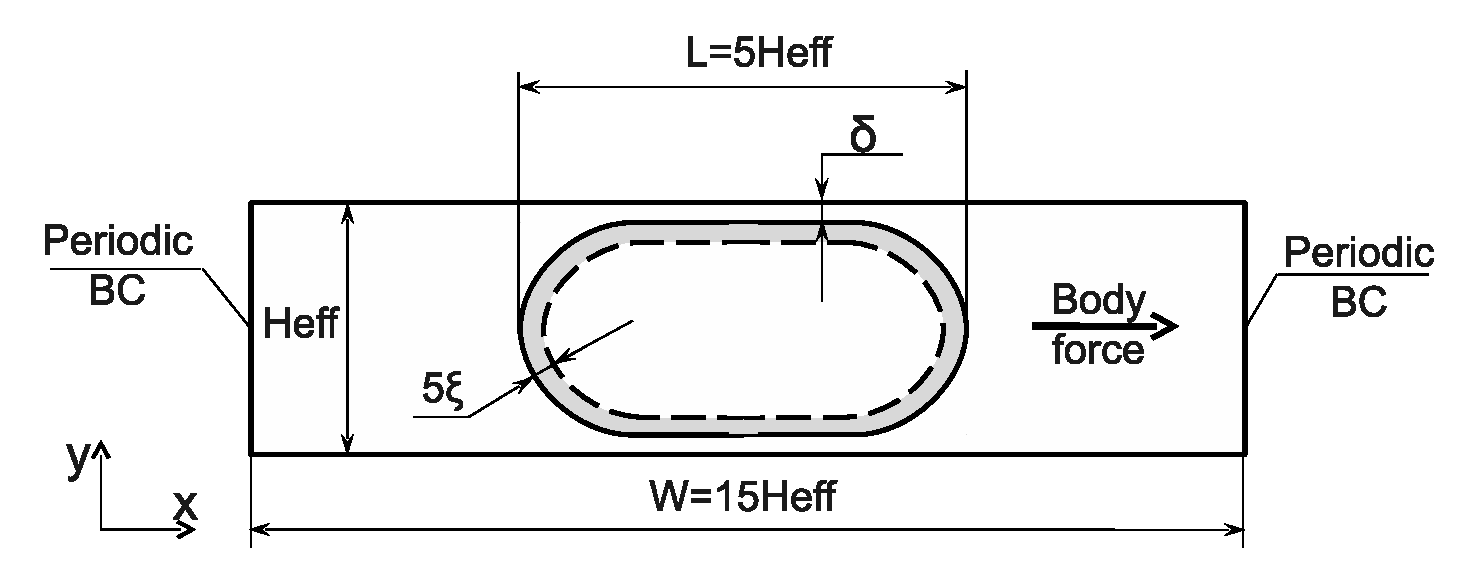
\includegraphics[width=\textwidth]{Figures/benchmark_new.eps}\\
\\
\\
\\
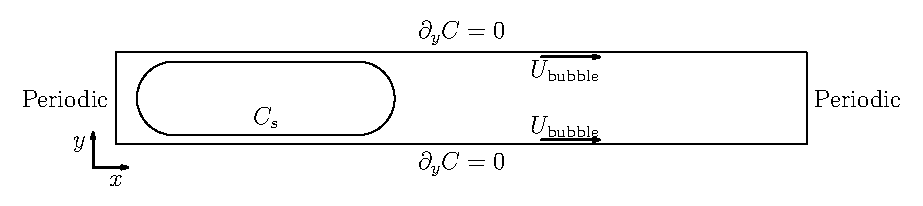
\includegraphics[width=\textwidth]{Figures/benchmark_periodic.eps}
\caption{The two-dimensional benchmarks for the hydrodynamics (top) and the mass transfer
coefficient (bottom). \label{fig:benchmark}}
\end{figure}

\section{Parameters choice}
In what follows we want to address the following empirical correlation addressed in the recent
publication by \citet{yue-mass}:
\begin{equation}
k_L a=\frac{2}{d_h} \Bigl(\frac{D
U_{\mathrm{bubble}}}{L_{\mathrm{bubble}}+L_{\mathrm{slug}}}\Bigr)^{0.5}
\Bigl(\frac{L_{\mathrm{bubble}}}{L_{\mathrm{bubble}}+L_{\mathrm{slug}}}\Bigr)^{0.3}.
\end{equation}
This correlation is within $10\%$ accuracy for experimental results within the following range of
parameters: $0.4\,\mathrm{m/s}<U_{\mathrm{bubble}}<2\,\mathrm{m/s}$,
$1.4<\frac{L_{\mathrm{bubble}}}{d_h}<6.3$, $1<\frac{L_{\mathrm{slug}}}{d_h}<3.2$, $d_h = 400
\mathrm{\mu m}$.

For long slug lengths in circular capillaries the folowing correlation is derived by
\citet{bercic-mass}:
\begin{equation}
k_L a = \frac{0.111
(U_{\mathrm{gas}}+U_{\mathrm{liq}})^{1.19}}{\bigl((1-\varepsilon_{\mathrm{gas}})(L_{\mathrm{bubble}}
+L_ {\mathrm{slug}} )\bigr)^{0.57} },
\end{equation}
where $\varepsilon_{\mathrm{gas}}=\frac{U_{\mathrm{gas}}}{U_{\mathrm{bubble}}}$ is the gas holdup,
$U_{\mathrm{gas}}$ is the superficial gas velocity, and $U_{\mathrm{liq}}$ is the superficial
liquid velocity. The superficial liquid velocity is calculated with the steady state condition in
the middle of the slug as:
\begin{equation}
U_{\mathrm{liq}}=\frac{\oint U \mathrm{d}A}{A}.
\end{equation}
The superficial liquid velocity can be calculated through the calculated bubble volume and gas
holdup:
\begin{equation}
\begin{aligned}
&\varepsilon_{\mathrm{gas}}=\frac{\text{bubble area}}{15 H^2}\\
&U_{\mathrm{gas}}=\varepsilon_{\mathrm{gas}} U_{\mathrm{bubble}}
\end{aligned}
\end{equation}
 

In their experiments \citeauthor{bercic-mass} dealt with long slug lengths.
Thus, they concluded that the mass transfer from bubble caps was predominant.

\citet{vanbaten-circular} performed numerical simulations for circular capillaries by assuming that
there is a separate contribution of the liquid film and the bubble caps to mass transfer. Their
correlation is as:
\begin{equation}
k_L a = \frac{2}{\sqrt{\pi}}\sqrt{\frac{D U_{\mathrm{bubble}}}{(L_{\mathrm{bubble}}-d_h)}}
\frac{4(L_{\mathrm{bubble}}-d_h)}{d_h(L_{\mathrm{bubble}}+L_{\mathrm{slug}})}+2\frac{\sqrt{2}}{\pi}
 \sqrt{\frac{D U_{\mathrm{bubble}}}{d_h}} \frac{4}{(L_{\mathrm{bubble}}+L_{\mathrm{slug}})}
\end{equation}
This correlation is valid for short contact times, when the mass transfer is important from bubble
caps as well as from the film. Short contact times are defined through Fourier number as:
\begin{equation}
Fo=\frac{D t_{\mathrm{film}}}{\delta^2},
\end{equation}
where $t_{\mathrm{film}}=\frac{L_{\mathrm{film}}}{U_{\mathrm{bubble}}}$ is the time exposure of the
bubble while it propagates through distance $L_{\mathrm{film}}$. 

Our goal is to compare numerical simulations with given correlations.

\section{Mass transfer}
The mass transfer is characterized by non-dimensional numbers as Schmidt number (viscous diffusion
rate over the mass diffusion rate), the Peclet number (convection over diffusion) and the Sherwood
number (convection mass transfer over the diffusion mass transfer):
\begin{equation}
\begin{aligned}
&Pe=\frac{U L}{D}\\
&Sh=\frac{K L}{D}\\
&Sc=\frac{\nu}{D}\\
\end{aligned}
\end{equation}

As far as parameters of the lattice Boltzmann system are not connected with real ones, one needs to
match the non-dimensional parameters with physical one.  One of the particular examples is the
work by \citet{bercic-mass} who used the methane dissolution to characterize the mass transfer for
bubble train flow. Thus, assumption for periodic boundary conditions stays. 

In what follows we will perform the matching of obtained hydrodynamics results
\cite{kuzmin-binary2d} with physical ones from experiment of \citet{bercic-mass}. The diffusion
coefficient of the methane under standard conditions \cite{methane-properties} is
$1.84\times 10^{-5} \mathrm{cm}^2/\mathrm{s}$. The diameters of capillaries were as $1.5$, $2.5$ and
$3.1$ $\mathrm{mm}$. For simplicity reasons we will choose the diameter of capillary as $1.5\,
\mathrm{mm}$. 
We will match parameters through given non-dimensional numbers. From the hydrodynamics
simulations the following parameters supplied:
\begin{equation}
\begin{aligned}
Ca=\frac{U \mu_{\mathrm{liq}}}{\gamma}\\
Re=\frac{\rho_{\mathrm{liq}} U L}{\mu_{\mathrm{liq}}}.
\end{aligned}
\end{equation}
From these two equation one can obtain the physical velocity obtained from non-dimensional numbers:
\begin{equation}
\begin{aligned}
Ca\cdot Re= \frac{\rho_{\mathrm{liq}} U^2 L}{\gamma}\\
U=\sqrt{\frac{Ca\,Re\,\gamma}{\rho_{\mathrm{liq}}L}}
\end{aligned}
\end{equation}

Assuming that the surface tension of water is $0.0728\,\mathrm{N/m}$, the density is
$1000\,\mathrm{kg/m^3}$,the hydraulic diameter of the channel to be $1.5\,\mathrm{mm}$ one can
calculate the physical velocity of the bubble.
Table \ref{table:twod:simulations} represents the number of simulations runs for the grid as
$202\times 3002$ and its nondimensional parameters. One can see that velocity is quite reasonable
as \citet{bercic-mass} declared that experiments were conducted for velocities in the ranges of
$0.01$ to $0.4\,\mathrm{m}/\mathrm{s}$ but for less capillary numbers. 
\begin{table}
\begin{tabularx}{\textwidth}{|X|X|X|X|X|X|}
$Ca$    &$Re$     &$U_{LB}$ &$\delta$&$\varepsilon_{\mathrm{gas}}$
&$U_{\mathrm{phys}}\mathrm{m/s}$\\
$0.026$ &$0.449$  &$0.0014$ &$0.040$ &$0.306$ &$0.023$   \\ 
$0.047$ &$0.820$  &$0.0027$ &$0.058$ &$0.293$ &$0.043$   \\ 
$0.080$ &$1.378$  &$0.0045$ &$0.085$ &$0.280$ &$0.073$ \\
$0.065$ &$1.126$  &$0.0037$ &$0.076$ &$0.266$ &$0.059$      \\
$0.222$ &$3.807$  &$0.0125$ &$0.122$ &$0.253$ &$0.202$  \\
$0.479$ &$8.222$  &$0.0271$ &$0.151$ &$0.249$ &$0.437$  \\
$0.736$ &$12.617$ &$0.0416$ &$0.164$ &$0.236$ &$0.671$  \\ 
$0.989$ &$16.960$ &$0.0559$ &$0.172$ &$0.230$ &$0.902$  \\
\end{tabularx}
\caption{Two-dimensional simulations for different
capillary numbers. \label{table:twod:simulations}}
\end{table}

\section{Lattice Boltzmann implementation}
For the lattice Boltzmann implementation we took $\omega=1.99$ which results in the following
lattice Boltzmann diffusivity parameter:
\begin{equation}
\begin{aligned}
&D=\frac{1}{3}\Bigl(\frac{1}{\omega}-\frac{1}{2}\Bigr)\\
&D=0.0008375
\end{aligned}
\end{equation}
In terms of Schmidt number (taking the liquid viscosity in former simulations as $\frac{2}{3}$) that
can result in:
\begin{equation}
\begin{aligned}
&Sc=\frac{\nu_{\mathrm{liq}}}{D}\\
&Sc=796\\
\end{aligned}
\end{equation}
Taking the water as $8.9 \times 10^{-4}\,\mathrm{Pa\cdot s}$ or kinematic viscosity as $8.9 \times
10^{-7} \,\mathrm{m^2/s}$ and the Schmidt number as $796$ that results in the following quantity:
\begin{equation}
D=1.118\times 10^{-5}\,\mathrm{cm^2/s},
\end{equation}
which is less than the diffusivity of the methane $1.84\times 10^{-5}\,\mathrm{cm^2/s}$ but is
physical. After calculation of physical parameters one can calculate characteristics for the mass
theoretical mass transfer. Table \ref{table:lengths} gives nondimensional and physical lengths of a
bubble and a slug.
\begin{table}
\begin{tabularx}{\textwidth}{|X|X|X|X|X|X|}
\hline
$Ca$&Bubble length& Slug Length&
$U_{\mathrm{gas}}\,\mathrm{m/s}$&$U_{\mathrm{liq}}\,\mathrm{m/s}$&$a,\,\mathrm{m^{-1}}$\\
\hline
$0.026$&$5.225$&$9.775$ &$0.0070$ &$0.0209$&$2.5538$\\
$0.047$&$5.22$ &$9.78$  &$0.0126$ &$0.0379$&$2.5431$\\
$0.080$&$5.215$&$9.785$ &$0.0204$ &$0.0615$&$2.5326$\\
$0.065$&$4.965$&$10.035$&$0.0157$ &$0.0504$&$2.4142$\\
$0.222$&$5.25$ &$9.75$  &$0.0511$ &$0.1560$&$2.5253$\\
$0.479$&$5.565$&$9.435$ &$0.1089$ &$0.3155$&$2.6518$\\
$0.736$&$5.51$ &$9.49$  &$0.1584$ &$0.4677$&$2.6269$\\
$0.989$&$5.505$&$9.495$ &$0.2074$ &$0.6190$&$2.6340$\\
\hline
\end{tabularx}

\caption{The nondimensional (scaled to the height of the channel) lengths for the same
lattice Boltzmann simulations as in Table \ref{table:twod:simulations}. As well superficial
gas-liquid velocities are presented.\label{table:lengths}}
\end{table}

The literature correlations of mass transfer dependence on the bubble velocities are presented in
Fig. \ref{fig:mass:transfer:theoretical}. Note, that the correlations presented in
Fig.\ref{fig:mass:transfer:theoretical} are used primarily for circular capillaries
(\citeauthor{vanbaten-circular,bercic-mass}) and for square capillaries (\citeauthor{yue-mass}). We
adapt these results for flow between parallel plats by using hydraulic
diameter \cite{bercic-mass} which can be calculated as:
\begin{equation}
d_h = \lim_{W\to\infty}\frac{4A}{P}=\lim_{W\to\infty}\frac{4 W\,H}{2(W+H)}=2 H.
\end{equation}
\begin{figure}[htb!]
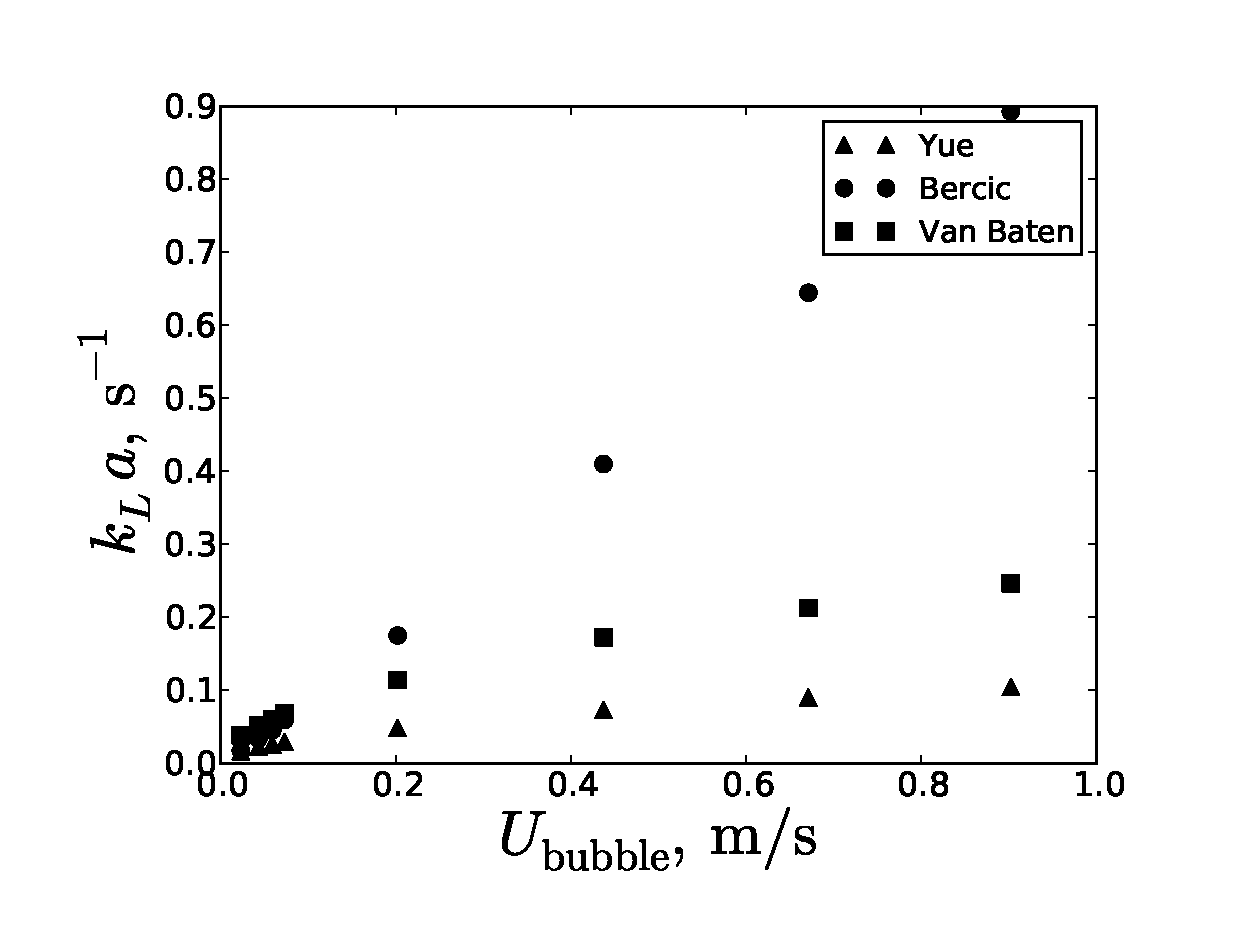
\includegraphics[width=\textwidth]{Figures/theoretical_correlations.eps}
\caption{The literature correlations by various authors. One
can see the large deviation among them.\label{fig:mass:transfer:theoretical}}
\end{figure}

The volumetric mass transfer coefficient is calculated according to the work of
\citet{vanbaten-circular}. The concentration flux is calculated as the difference between overall
average concentration taken in the whole domain ($C_{overall}=\int_{V} C \mathrm{d}V /V$) 
{\color{red} (In this particular moment I don't know whether to take the Volume of whole domain or
just the liquid phase. I will go for whole domain.)}
at time
$t_1$ and time $t_2$ divided on the time difference $t_2-t_1$. Then the volumetric mass transfer
coefficient is calculated as:
\begin{equation}
\label{main:simulation:equation}
k_L a=\frac{\text{Flux}}{C_s-C_{outlet}} \frac{\text{bubble surface area}}{\text{unit cell volume}},
\end{equation}
where $C_{outlet}=\int{C U_{outlet}\mathrm{d}A}/\int{U_{outlet}\mathrm{d}A}$. 
{\color{red} Do not understand why we need this ratio bubble surface area/unit cell volume. In this
case the dimensional units do not coincide. In the calculations I will avoid it until further
clearance.}
To properly do
non-dimensioanalization one needs to insure the time conversion factor when the flux is calculated
inside the lattice Botlzmann system. The time conversion can be easily obtained:
\begin{equation}
\begin{aligned}
&U_{LB}=U_{phys}\frac{\Delta t}{\Delta x}\\
&\Delta t=\frac{U_{LB}}{U_{phys}}\Delta x\\
&\Delta t=\frac{1.5\,\mathrm{mm}}{200} \frac{0.0559}{0.902\,\mathrm{m/s}}=4.64\times
10^{-7}\,\mathrm{s} 
\end{aligned}
\end{equation}

The bubble surface length is the perimeter of the bubble in two-dimensional space and it is
calculated with the extraction of the bubble countour and representing it with the polygon. After
that the calculated perimeter is the effective summation of line lengths and ca be represented as:
\begin{equation}
P=\sum_i{\sqrt{(x2_i-x1_i)^2+(y2_i-y1_i)^2}},
\end{equation}
where the index $i$ represents the polyline consisting of two points $(x1,y1)$ and $(x2,y2)$.

The corresponding volumetric mass transfer coefficients depending on the velocity are indicated in
Table \ref{table:lengths}.


\section{Simulation results}
\subsection{Steady-state}
Using Eq.\ref{main:simulation:equation} we calculated the mass transfer coefficient. One can see
the plots for the mass transfer coefficient versus time in Fig. \ref{fig:steady:state}. We state as
a steady-state condition the average of  
\begin{figure}
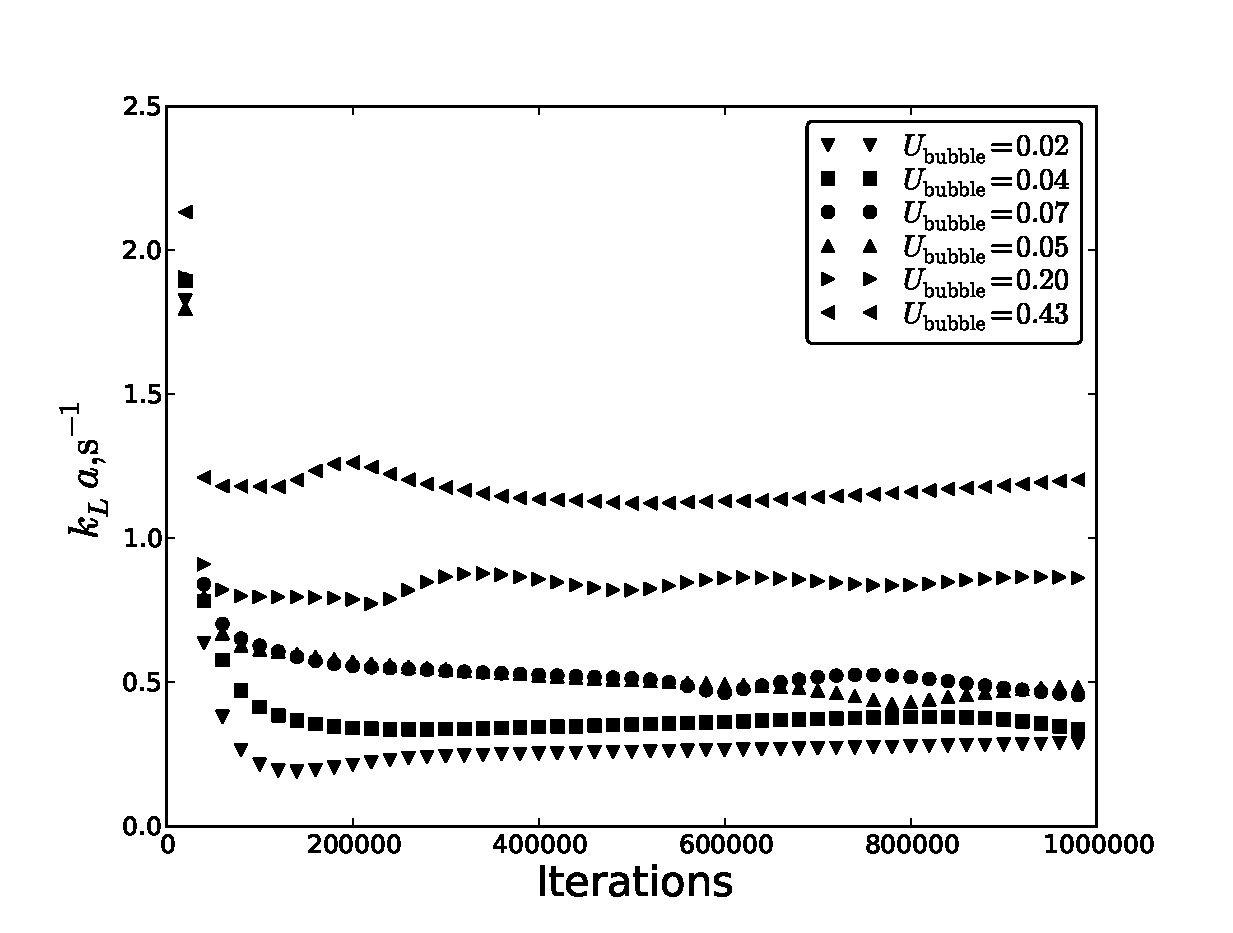
\includegraphics[width=\textwidth]{Figures/steady_state.eps}
\caption{The mass transfer coefficient vs. time iterations. One can see that the pseudo steady
state can be reached after $500000$. The mass transfer coefficient is taken as the average from
$500000$ to $1000000$.\label{fig:steady:state}}
\end{figure}


\section{To revise:}
Then the diffusion penetration length is:
\begin{equation}
\delta_{penetration}=\sqrt{D t_{film}}=\sqrt{\frac{D L_{bubble}}{U_{bubble}}}.
\end{equation}
The bubble length is $5$ of diameters. Thus, the bubble length is $7.5\,\mathrm{mm}$. Therefore:
\begin{equation}
\delta_{penetration}=\sqrt{\frac{1.84 10^{-9} \mathrm{m^2/s} 7.5 10^{-3} \mathrm{m}}{4.3 \time
10^{-2}\mathrm{m/s}}}=1.8 \times 10^{-5}
\end{equation}
With the given value of $200$ nodes to resolve the diameter for the given simulation, that results
in $2.4$ nodes, which is small but considerable number to conduct the simulation.
Foirier number which is defined as:
\begin{equation}
Fo=\frac{D t_{film}}{\delta_{film}^2}=\frac{1.84\times 10^{-9} 0.1744}{\times
(8.7\times10^{-5})^2}=0.0423
\end{equation}
As it is indicated by \citet{vanbaten-circular} the Fourier number $Fo<0.1$ stays for short
contact, the film is unsaturated. 
Thus, one can calculate the corresponding parameters:
\begin{equation}
Pe_{min}=\frac{10^{-2} 1.5 10^{-3}}{1.84  10^{-9}}=0.81 \times 10^{4}\gg 1
Sc_{min}=\frac{10^{-6}}{1.84 10^{-9}}=543,
\end{equation}
which imply the Reynolds number to be as:
\begin{equation}
Pe=Re Sc,\,Re=Pe/Sc=14.91
\end{equation}

The Schmidt number $Sc \approx 500$ states for dye in the liquid and assumes the dominance of
convection over diffusion. In terms of the lattice Boltzmann system, the liquid viscosity equals to
$\frac{1}{3}(\tau_{liq}-\frac{1}{2})=\frac{2}{3}$. That means that the relaxation rate for the
advection-diffusion equation should be as:
\begin{equation}
\frac{1}{3}\Bigl(\tau_{\phi}-\frac{1}{2}\Bigr)=\frac{\nu}{Sc}\\
\tau_{\phi}=0.50368,
\end{equation}
which is hard to simulate with the lattice Boltzmann equation, but possible . As it was discussed
\cite{giavedoni-numerical} the inertia can be neglected for the Reynolds number $Re<70$ for bubble
configuration, but not for the hydrodynamics simulations.

The easy way to do is not to match the Peclet number $Pe$ along with the Reynolds number, leaving
only matching the Schmidt number. However, the thorough study needs to be conducted to perform the
matching parameters as $Ca$, $Re$, $Sc$ and $Pe$ numbers. 

If we match only the Peclet number then the Reynolds number can be changed as to adjust the
velocity multiplied on coefficient, keeping Reynolds number small and anticipating results to see.


\appendix

\section{Boundary conditions}
In what follows we will examine different LBM implementations:
\begin{description}
 \item[BB conditions] The walls can be treated via the simple bounce back rule:
\begin{equation}
f_{\bar{i}B}=f_{iF},\text{ for } \forall i,
\end{equation}
where $B$ is the boundary node with coordinates $\bm{r_F}+\bm{c_i}$, $F$ is the fluid node. This
will fulfill the macroscopic conditions as:
\begin{equation}
J_{fluid}= \sum_{c_i\cdot n>0}{f_i c_i}=J_{wall},
\end{equation}
which is in turn represents the following boundary condition:
\begin{equation}
\partial_n J_n=\partial_n C u_n = u_n \partial_n C=0
\end{equation}

The walls can be treated through simmetric boundary conditions as well, which are really close to
bounce-back formulation. In this case one can insure that the concentration values at the wall and
at the fluid equal to each other. 

For the constant concentration at the bubble surface one can use the pressure anti
bounce-back conditions
\cite{ginzburg-boundary-main}:
\begin{equation}
f_{iB}=-f^{*}_{iF}+2 e_i(W),
\end{equation}
where the subscript $*$ stands for after-collision population, $W$ stands for the wall
concentration to be imposed.
\item[Inamuro conditions] Inamuro boundary conditions impose strict conservation of the population
by utilizing diffuse interface kinetic boundary approach \cite{inamuro-scalar-boundary}. The
unknown populations $f_i=w_i \rho^{\prime}\text{ for } \bm{c_i}\cdot \bm{n}>0$ are prescribed
through the equilibrium conditions, where $\rho^{\prime}$ is an unknown parameter.Then the
prescribed wall condition is as: 
\begin{equation}
\rho^{\prime}=\frac{\rho_{w}-\sum_{i,\bm{c_i}\cdot\bm{n}\leq0}
f_i}{\sum_{i,\bm{c_i}\cdot\bm{n}>0}w_i}
\end{equation}
For the zero flux on the wall one can use another equation:
\begin{equation}
\rho^{\prime}=-\frac{i,\bm{c_i}\cdot\bm{n}\leq0}{\sum_{i,\bm{c_i}\cdot \bm{n}}{w_i \bm{c_i}\cdot
\bm{n}}}.
\end{equation}
\end{description}


\section{TRT $D2Q9$ model. Equilibrium functions}
One of the advantages of $D2Q9$ TRT model in comparison with $D2Q5$ usually used for simulations of
the advection-diffusion model is that $D2Q9$ is able to reduce numerical diffusion from diagonal
and non-diagonal diffusion tensor components \cite{kuzmin-stability-optimal}.

In
comparison with the BGK collision operator the TRT collision operator \cite{ginzburg-boundary-main}
decomposes the populations and the equilibrium
distribution into the symmetric and antisymmetric parts:
\begin{equation}
\label{trtdecomp}
f^{\pm}_i=\frac{f_i\pm f_{\bar{i}}}{2}\;,\; 
{eq_i}^{\pm}=\frac{eq_i\pm eq_{\bar{i}}}{2}\;,
\end{equation}
where $\bar{i}$ is the opposite direction to the $i$-th direction.
The collision is performed with two independent relaxation rates for 
symmetric and antisymmetric modes:
\begin{equation}
\label{trt}
\begin{aligned}
&f_i^{*}(\bm{x},t)=f_i(\bm{x},t)-\omega_{+} (f_i^{+} - eq_i^+)-\omega_{-}
(f_i^{-} -
eq_i^-)\\
&f_i(\bm{x}+\bm{c_i},t+1)=f_i^{*}(\bm{x},t).
\end{aligned}
\end{equation}
Note that the BGK collision operator is the particular subclass of the TRT relaxation operator with
$\omega_{+}=\omega_{-}$. In comparison with the BGK collision operator,
the TRT collision operator has the additional degree of freedom. Thus, the TRT operator then
introduces
so-called magic (free) parameter
$\Lambda=\Bigl(\frac{1}{\omega_{+}}-\frac{1}{2}\Bigr)\Bigl(\frac{1}{\omega_{-}}-\frac{1}{2}\Bigr)$. 
This free parameter controls the effective location of the bounce-back
walls \cite{ginzburg-multireflection}, second-order accuracy of
boundary \cite{ginzburg-boundary-main} and interface schemes \cite{ginzburg-discontinious}, 
spatial accuracy \cite{ginzburg-recurrence,servan-trt-stability},
consistency \cite{ginzburg-brinkman} and, to some extent,
stability \cite{kuzmin-stability-optimal,kuzmin-d1q3,servan-trt-stability}.
In particular, $\Lambda=\frac{1}{4}$ achieves the optimal stability for the
linear advection-diffusion isotropic equation \cite{kuzmin-stability-optimal}. 

The equilibrium functions for $D2Q9$ TRT model are represented as \cite{kuzmin-stability-optimal}:
\begin{equation}
\begin{aligned}
&eq_i^{+}=eq_i^{(m)}+g^{(u)} eq_i^{(u)}\\
&eq_i^{(m)}=t_i^{(m)} c_e+ eq_i^{(a)}\\
&eq_i^{(u)}=t_i^{(u)} \frac{u_x^2+u_y^2}{2}+\frac{u_x^2-u_y^2}{4} p_i^{(xx)}+g_{xy}^{(u)}\frac{u_x
u_y}{4} p_i^{xy}\\
&eq_i^{(a)}=\frac{D_{xx}-D_{yy}}{4} p_i^{xx}+\frac{D_{xy}}{4} p_i^{(xy)},
\end{aligned}
\end{equation}
where $p_i^{(xx)}=c_{ix}^2-c_{iy}^2$ and $p_i^{(xy)}=c_{ix} c_{iy}$. 

The following equilibrium functions solve the anisotropic advection-diffusion equation with the
following diffusion tensor:
\begin{equation}
D=
\begin{pmatrix}
D_{xx} + (g^{(u)}-1) u_x^2 & D_{xy}+(g_{xy}^{(u)}-1)u_x u_y\\
D_{xy} + (g_{xy}^{(u)}-1) u_x u_y& D_{yy}+(g^{(u)}-1) u_y^2 
\end{pmatrix}
\end{equation}
To consider the situation when the resolution is not needed to be changed in $x$ and $y$
directions, one can obtain that $D_{xx}=D_{yy}$. The cross-diagonal components of the diffusion
tensor are taken as zeros, i.e. $D_{xy}=0$. The numerical diffusion can be avoided by proper choice
of the equilibrium functions, i.e. $g_{xy}^{(u)}=g^{(u)}=1$.

As far as the simulated diffusion tensor is close to $0$ the stability limits restrict the velocity
amplitude to be simulated \cite{kuzmin-stability-optimal}. However, particular choice of weights
can drastically help. Fig. \ref{stability:d2q9} shows the stability limits for D2Q9 with removed
numerical diffusion and with it for two particular choices of weights.
\begin{figure}[htb!]
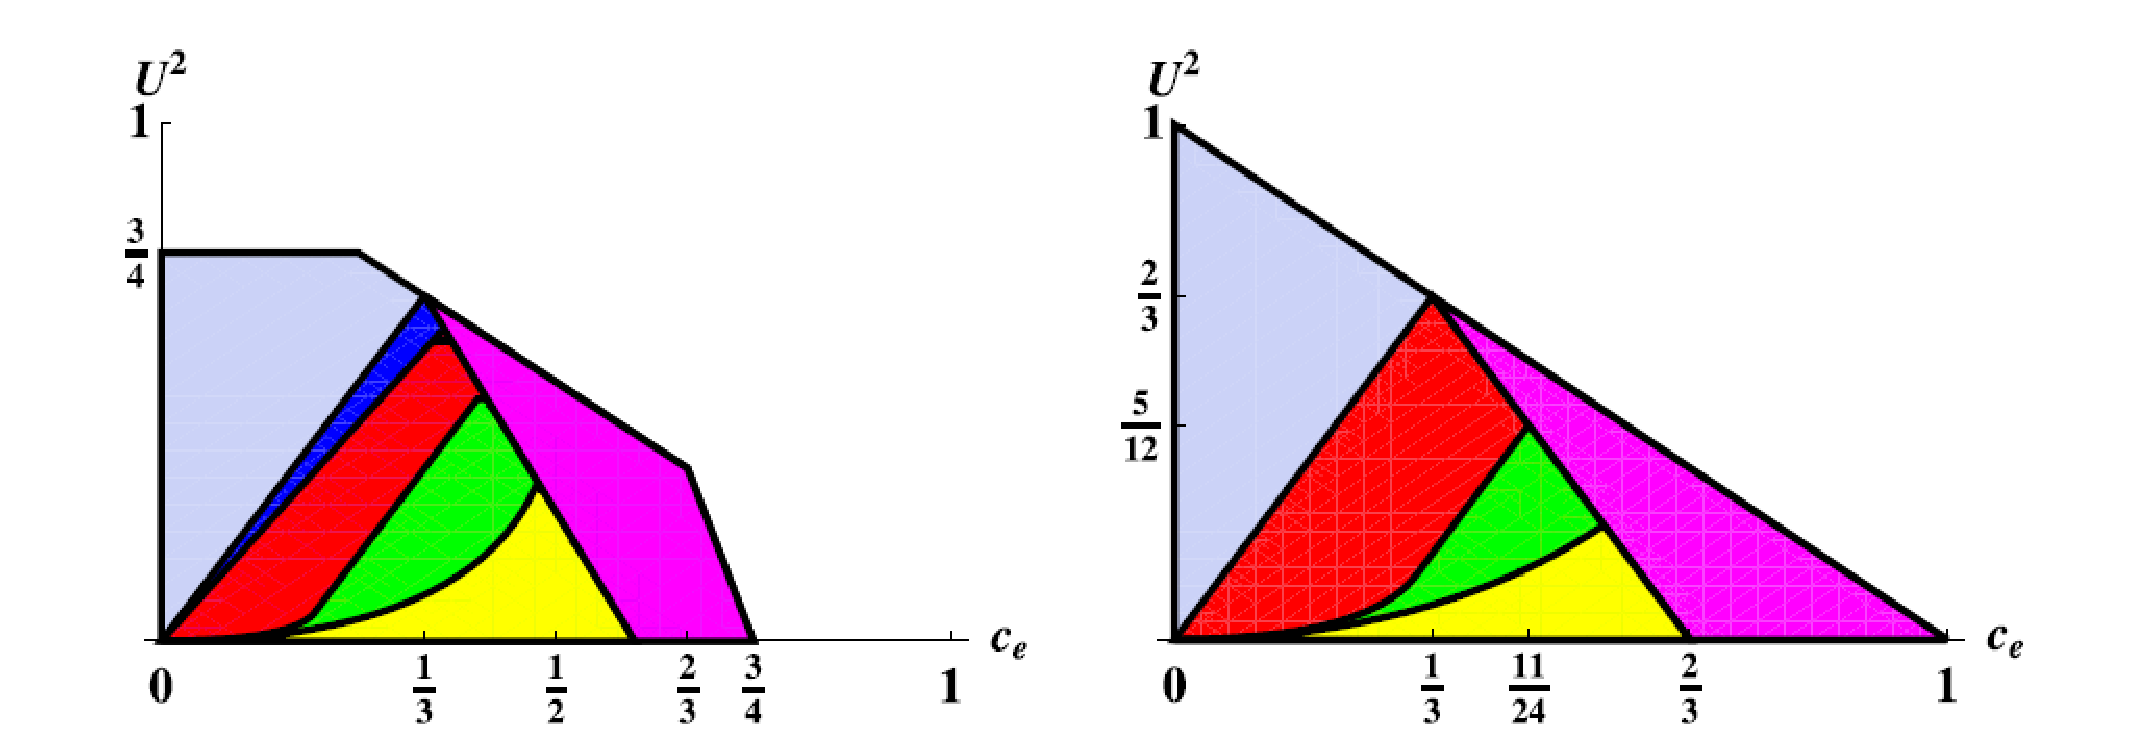
\includegraphics[width=\textwidth]{Figures/d2q9_stability.eps}
\caption{The non-negativity areas and stable sub-domains of the OTRT schemes ($\Lambda=\frac{1}{4}$)
are plotted for the $D2Q9$ (standard weights, left) and the $D2Q9$ (uniform weights, right) when the
numerical diffusion is removed, partially or completely. Two non-negativity areas where all the
equilibrium populations are positive have curvilinear boundaries: they are smaller when
$g^{(u)}_{xy}=0$ (yellow) and than when $g^{(u)}_{xy}=1$ (green+yellow). The non-negativity
condition is required by BGK collision operator. The stable sub-domains for $g^{(u)} = 1,
g^{(u)}_{xy} = 0$ are small (red+green+yellow) triangles. When the numerical diffusion is removed
the stable area is bounded by magenta and the (blue) domain above. The proper choice of weights can
allow to obtain  total triangle $0 \leq u_x^2+u_y^2 \leq 1−c_e$ (the
uniform weights only).
\label{stability:d2q9}}
\end{figure}

From here on we will use the standard weights as:
\begin{equation}
t_i^{(u)}=t_i^{(m)}=t_i^{(a)}=\Bigl\{0,\frac{1}{3},\frac{1}{3},\frac{1}{3},\frac{1}{3},\frac{1}{12},
\frac {1}{12},\frac{1}{12},\frac{1}{12}\Bigr\}
\end{equation}

\bibliographystyle{unsrtnat}
\bibliography{paper}

\end{document}
